\documentclass[a0paper,portrait]{baposter}


\usepackage[font=small,labelfont=bf]{caption} % Required for specifying captions to tables and figures
\usepackage{booktabs} % Horizontal rules in tables
\usepackage{relsize} % Used for making text smaller in some places
\usepackage{xcolor}
\usepackage{wrapfig}
\usepackage{ctable}
\usepackage[percent]{overpic}

\definecolor{bordercol}{RGB}{40,40,40} % Border color of content boxes
\definecolor{headercol1}{RGB}{159,188,191} % Background color for the header in the content boxes (left side)
\definecolor{headercol2}{RGB}{123,144,146} % Background color for the header in the content boxes (right side)
\definecolor{headerfontcol}{RGB}{0,0,0} % Text color for the header text in the content boxes
\definecolor{boxcolor}{RGB}{255,255,255} % Background color for the content in the content boxes

% amsmath packages
\usepackage{amsmath}
\usepackage{amsfonts}
\usepackage{amssymb}

\begin{document}

\background{% Set the background to an image (background.pdf)
\begin{tikzpicture}[remember picture,overlay]
\draw (current page.north west)+(-2em,2em) node[anchor=north west]
{
  
\includegraphics[height=1.06\textheight]{figures/background.pdf}
};
\end{tikzpicture}
}

\begin{poster}{
grid=false,
borderColor=bordercol, % Border color of content boxes
headerColorOne=headercol1, % Background color for the header in the content boxes (left side)
headerColorTwo=headercol2, % Background color for the header in the content boxes (right side)
headerFontColor=headerfontcol, % Text color for the header text in the content boxes
boxColorOne=boxcolor, % Background color for the content in the content boxes
headershape=roundedright, % Specify the rounded corner in the content box headers
headerfont=\Large\sf\bf, % Font modifiers for the text in the content box headers
textborder=rectangle,
background=user,
headerborder=open, % Change to closed for a line under the content box headers
boxshade=plain
}
{}
%----------------------------------------------------------------------------------------
%  TITLE AND AUTHOR NAME {{{1
%----------------------------------------------------------------------------------------
{\sf\bf
  \hspace*{-1em}
  Equation of motion coupled cluster theory \\
  using periodic boundary conditions
} % Poster title
{\vspace{.2em}\bf A. Gallo, F. Hummel and A. Gr\"uneis\\ % Author names
{\smaller\bf Max-Planck-Institute for Solid State Research, Stuttgart, Germany}\\  % Author affiliation
\vspace{-0.2em}
{\smaller\bf Institute for theoretical Physics, TU Wien, Vienna, Austria}\\  % Author affiliation
{\smaller\it a.gallo@fkf.mpg.de}  % Author affiliation
\vspace{-1cm}
}
%}}}1

%  Abstract {{{1  %
%%%%%%%%%%%%%%%%%%%
\begin{posterbox}[ name=introduction,column=0,span=3,row=0.03 ]{Introduction}

  Nitrogen Vacancy defects in diamond have become over the last years
an important candidate for a bulk room temperature quantum information processing device. 
In this poster we investigate the feasibility of approximate density functional theory calculations for describing optical and electronic properties for several 
vacancy-impurity complexes
in different carbon allotropes. 


\end{posterbox}
%}}}1

%  Variables {{{1  %
%%%%%%%%%%%%%%%%%%%%
\def\posterImageSize{0.95}
%}}}1

%  computational details Details {{{1  %
%%%%%%%%%%%%%%%%%%
\headerbox{Computational details}{
  name=computational-details,
  column=0,
  span=1,
  below=introduction}{

  \begin{itemize}
    \item
      Implementation in package \texttt{cc4s} (\textit{Coupled Cluster for
      solids})
    \item DFT and HF calculations performed with \texttt{VASP}
    \item Plane waves basis set
    \item Cyclops tensor framework (\texttt{CTF}) as a tensor contraction engine
  \end{itemize}

}
%}}}1

%  cc {{{1  %
%%%%%%%%%%%%%%%%%%%
\headerbox{Coupled-Cluster Ansatz}{
  name=coupled-cluster,
  column=0,
  row=0.03,
  below=computational-details}{
  \begin{itemize}
    \item
      Exponential \textit{Ansatz} for dynamic correlation
      %
      \[
        \left | \mathrm{CC} \right \rangle  = e^{\hat{T}} \left | 0 \right \rangle
      \]
      %
    where $ \left | 0 \right \rangle  $ is the one-particle vacumm.
    %
    \[
      \hat{T} =
      \underbrace{
      \sum_{a,i}^{}
        {\color{blue}t^{a}_{i} }
        \hat{a}^{\dagger}_{a} \hat{a}_{i}
      +
      \sum_{a,b,i,j}
        {\color{blue}t^{ab}_{ij} }
        \hat{a}^{\dagger}_{a} \hat{a}^{\dagger}_{b}
        \hat{a}_{j}           \hat{a}_{i}
      }_{\mathrm{CCSD}}
      + \cdots
    \]
    %
    \item
      Size consistency and extensivity
  \end{itemize}
}
% }}}1

%  Eq of motion cc {{{1  %
%%%%%%%%%%%%%%%%%%%
\headerbox{Equation of motion CC}{
  name=eomcc,
  column=0,
  row=0.03,
  below=coupled-cluster}{

  \begin{itemize}
    \item
      Linear \textit{Ansatz} on top of ground state coupled-cluster.
        $$
        \left | r_i \right \rangle =
        \hat{R} ^{(i)} e^{\hat{T}} \left | 0  \right \rangle
        $$
        $$
        \left \langle l_i \right | =
        \left \langle 0 \right | e^{-\hat{T}} \hat{L}^{(i)}
        $$
      where
        $$
          \hat{R} ^{(i)} = r _{0}
                         + r ^{a} _{i} \hat{c} ^{\dagger} _{a} \hat{c} _{i}
                         + r ^{ab} _{ij} \hat{c} ^{\dagger} _{a} \hat{c} ^{\dagger} _{b}
                                \hat{c} _{j} \hat{c} _{i}
                         + \ldots
        $$
        $$
          \hat{L} ^{(i)} = l _{0}
                         + l ^{i} _{a} \hat{c} _{i}^{\dagger} \hat{c} _{a}
                         + l ^{ij} _{ab}
                            \hat{c} _{j} ^{\dagger} \hat{c} _{i}^{\dagger}
                            \hat{c} _{a} \hat{c} _{b}
                         + \ldots
        $$

    \item
      Non-hermitian diagonalization problem of
        $ \bar{H} = e^{-\hat{T}} \hat{H} e^{\hat{T}}$

    \item
      Left and right eigenvectors $ \Rightarrow $ accessibility to calculate
      properties.

    \item
      Size consistency inherited from CC

  \end{itemize}

  \textbf{Davidson diagonalization}
  \begin{itemize}

    \item
      Get initial \textit{right} basis
      $ B = \left \{ b_{1}, \ldots, b_{k} \right \} $
      to obtain $ k $ excited states

    \item
      Compute reduced matrix and diagonalize
      $
        h_{ij} =
        \left \langle b_{i} \right | \bar H \left | b_{j} \right \rangle
      $

    \item
      Get $ k $ lowest eigenvalues and eigenvectors and compute corrections
      for them

    \item
      If the corrections are significant, add them to the basis

    \item
      Basis refreshment: at some iterations, the basis gets collapsed
      to have only $ k $ vectors

  \end{itemize}




}
% }}}1

%  Discussion Batom {{{1  %
%%%%%%%%%%%%%%%%%%%%%
\headerbox{The Boron atom: \textrm{UCCSD} }{
  name=discussion-batom,
  column=1,
  span=2,
  below=introduction
  }{
  \begin{minipage}{0.2\textwidth}
    \centering
    \includegraphics[height=1\textwidth]{figures/boron_orbitals/orbitals.pdf}
  \end{minipage}
  \begin{minipage}{0.75\textwidth}
    \begin{itemize}
      \item
        Open shell systems through \emph{uccsd} and \emph{eom-ccsd}.
      \item
        Benchmark of diagonalization procedures and convergence behaviour.
      \item
        155 unoccupied spin orbitals.
    \end{itemize}
  \end{minipage}
  \begin{center}
    \includegraphics[height=0.4\textwidth]{figures/boron_energies/plot.pdf}
  \end{center}
}
%}}}1

%  Discussion NV center {{{1  %
%%%%%%%%%%%%%%%%%%%%%
\headerbox{The $ NV^{-} $ centre }{
  name=discussion-nvcenter,
  column=1,
  span=2,
  below=discussion-batom
  }{
  \begin{minipage}{0.44\textwidth}
    \centering
    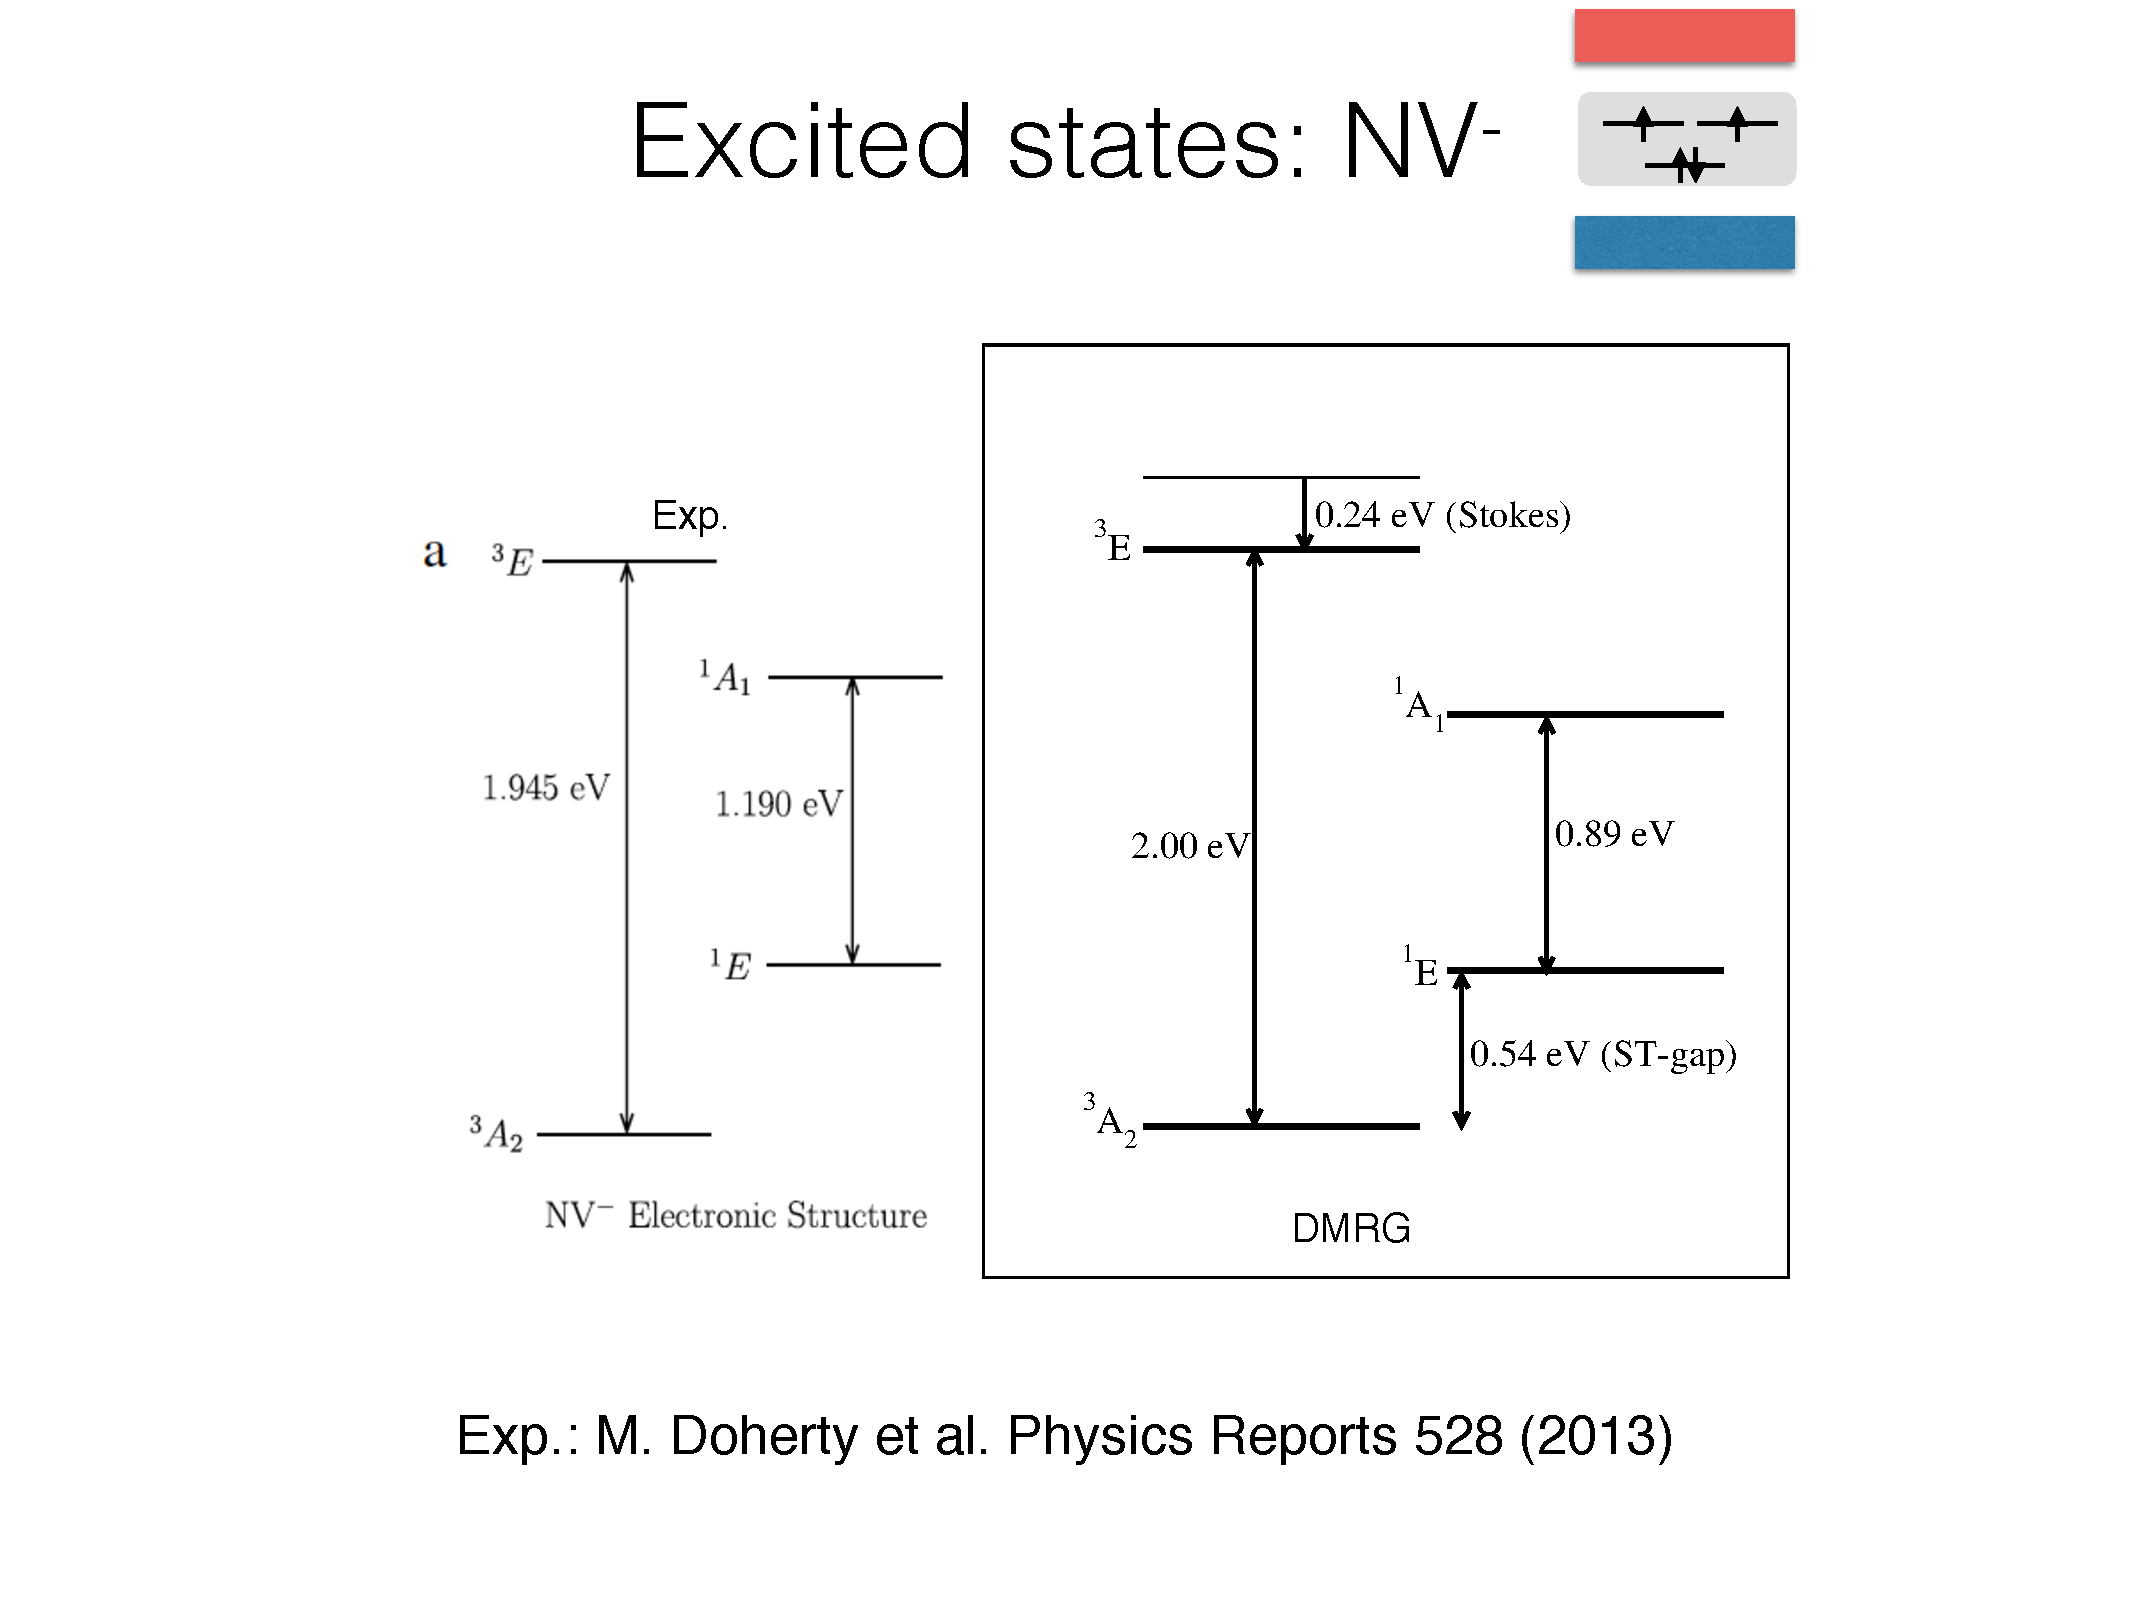
\includegraphics[width=0.5\textwidth, trim=220 200 570 220, clip]{figures/dmrg_results.pdf}
    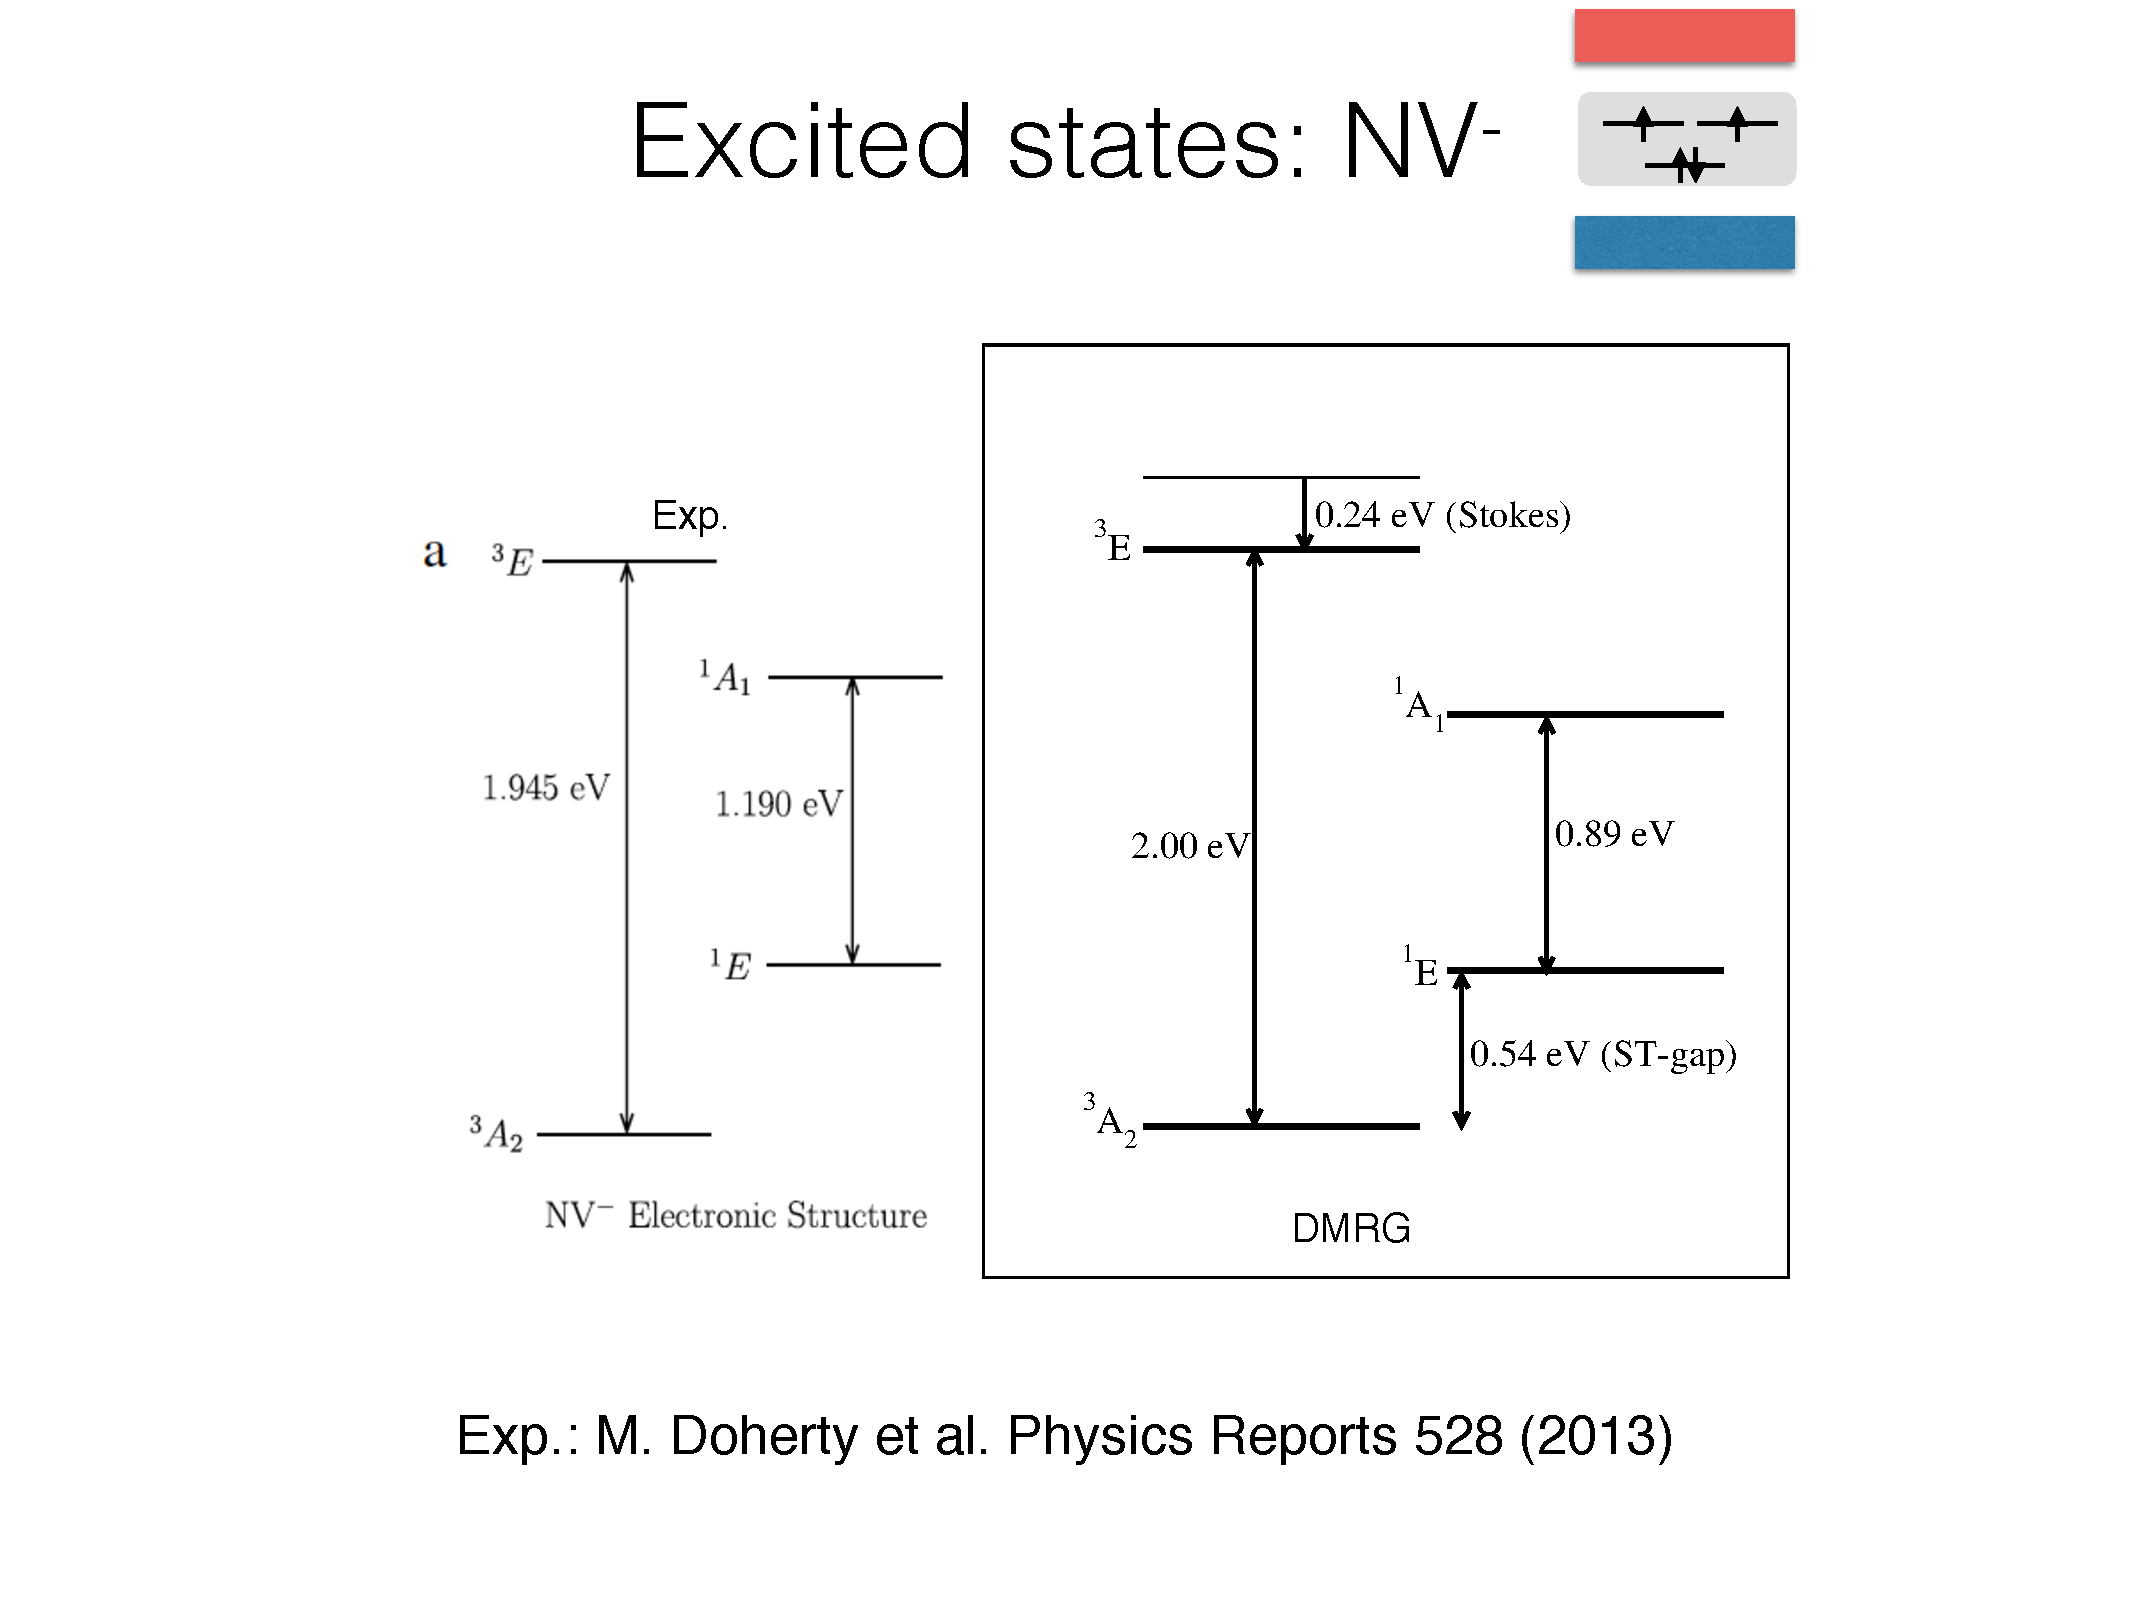
\includegraphics[width=0.6\textwidth, trim=500 200 190 200, clip]{figures/dmrg_results.pdf}
  \end{minipage}
  \begin{minipage}{0.2\textwidth}
    \centering
    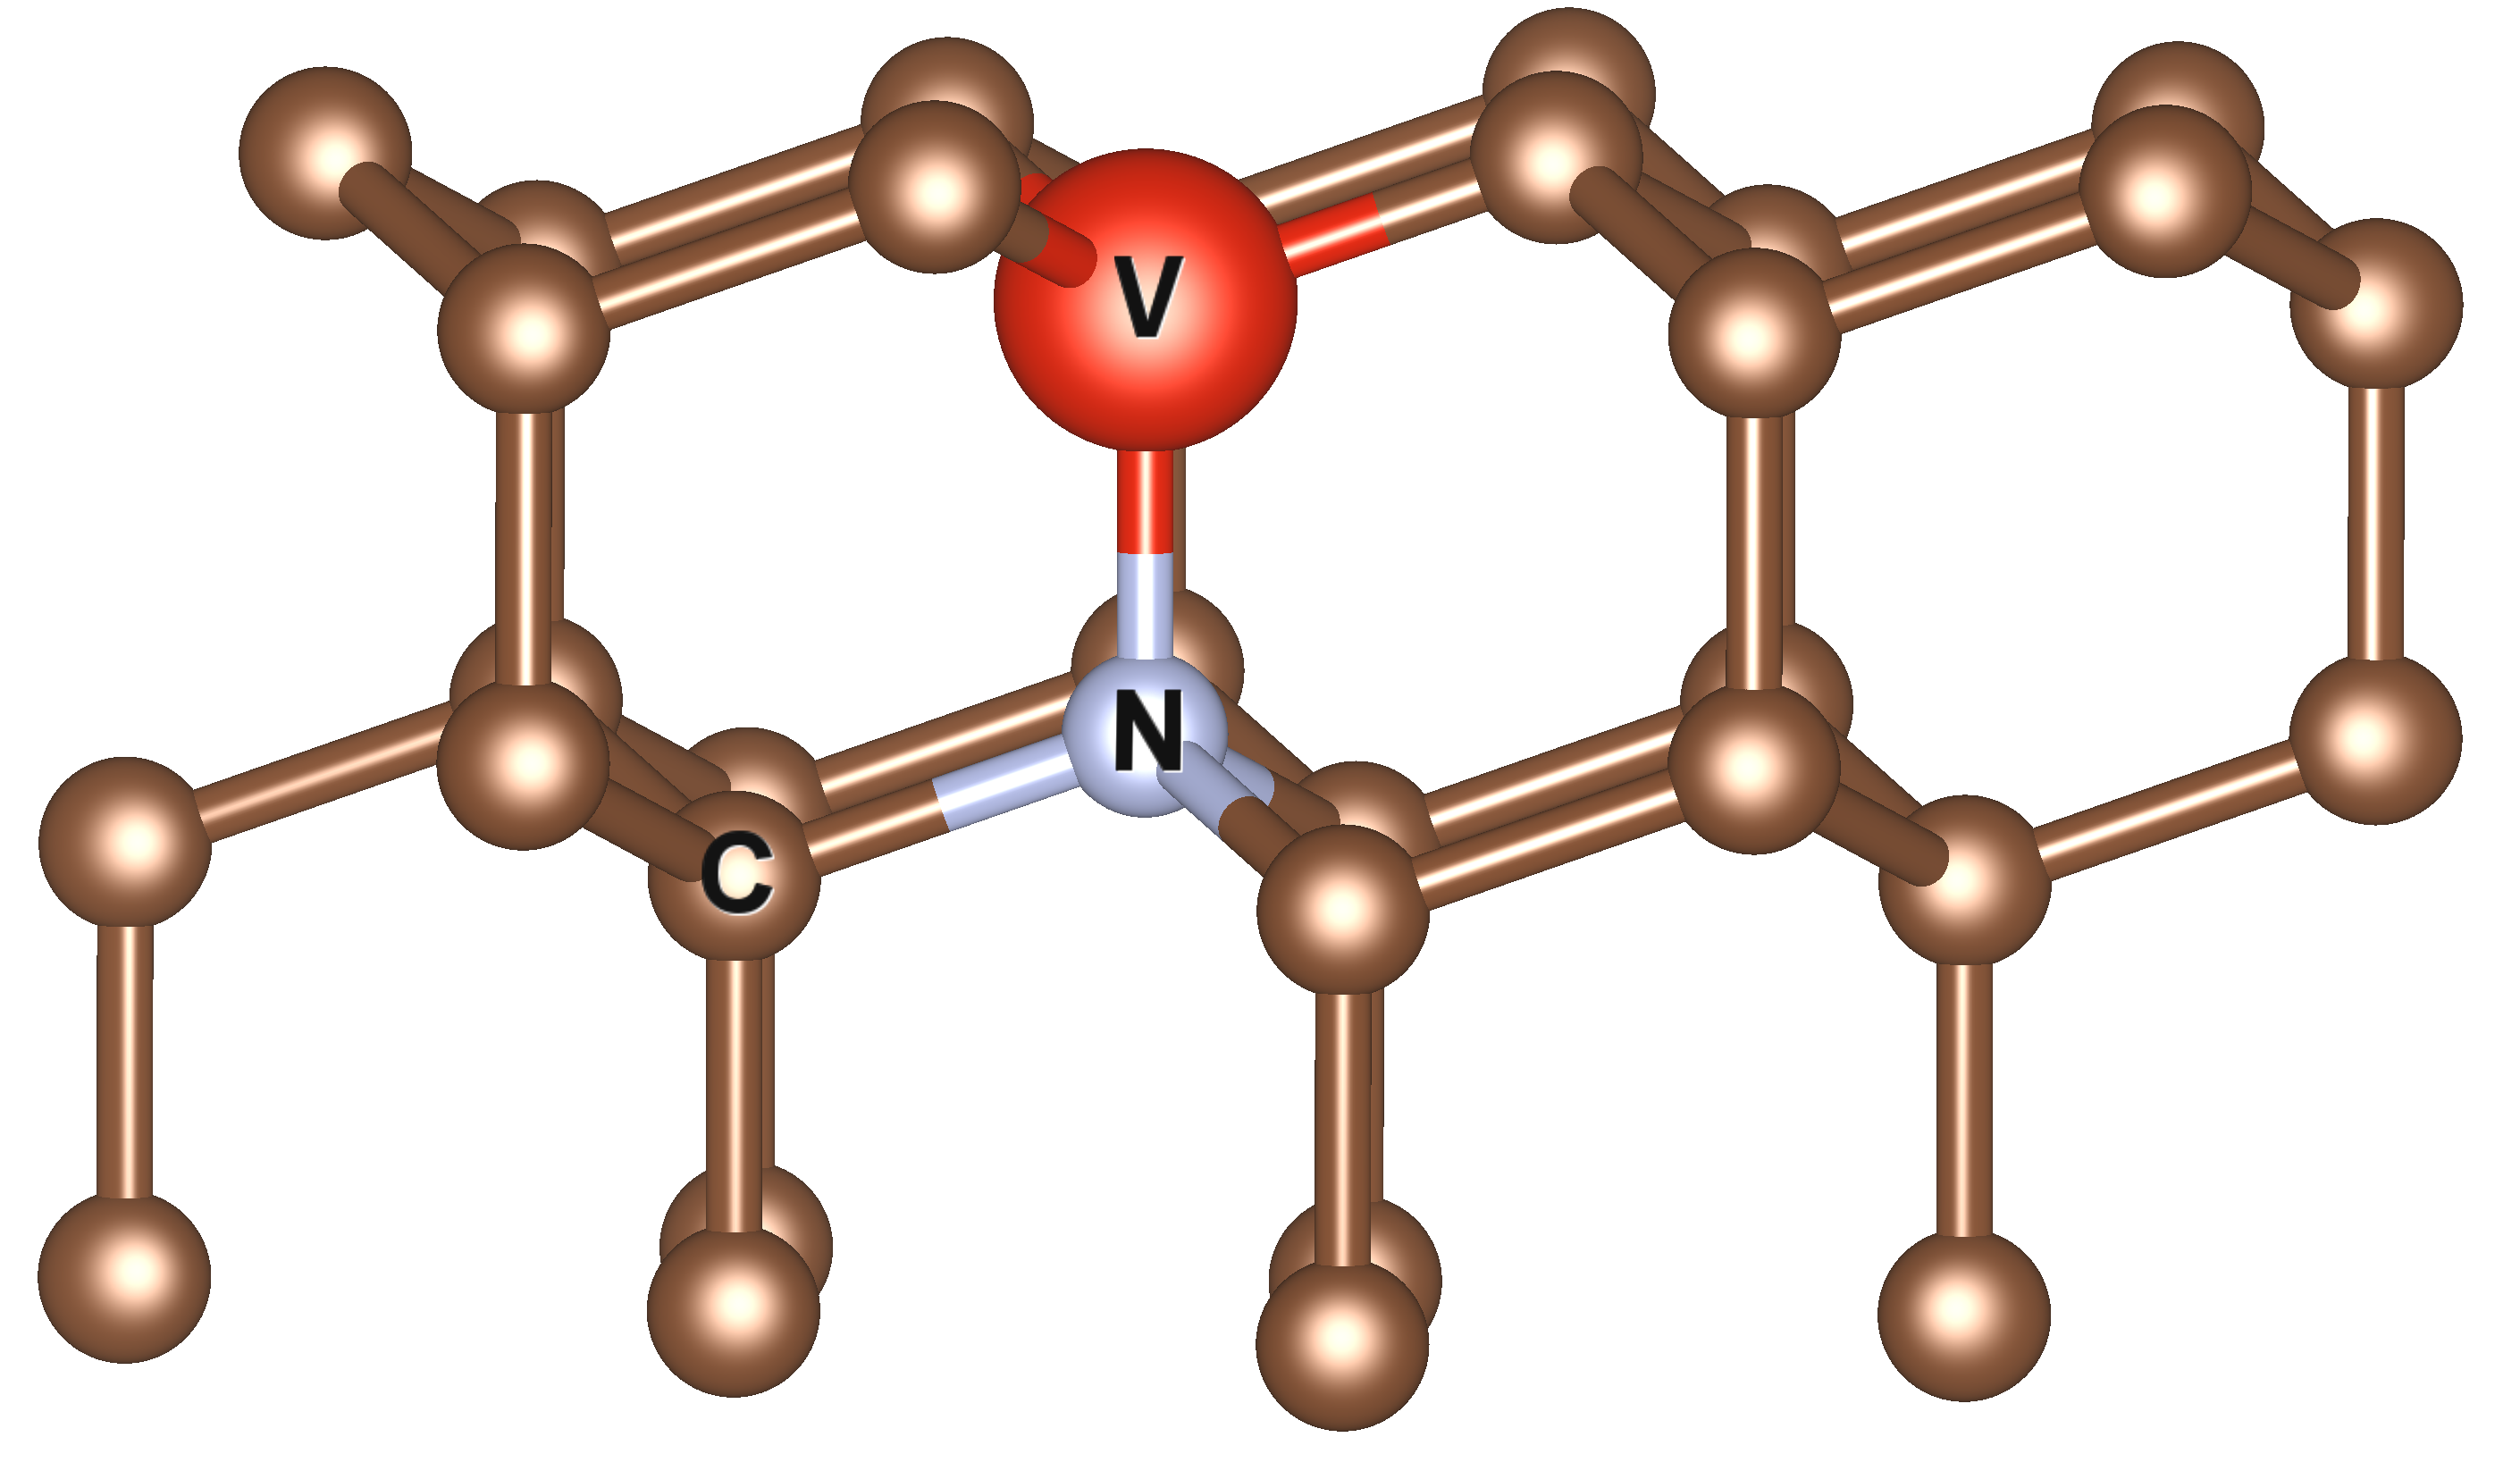
\includegraphics[height=1.3\textwidth]{figures/POSCAR_16_view.png}
    \includegraphics[height=1.7\textwidth]{figures/simple_orbital_pictures/basic_level_definition_with_spin_3.pdf}
  \end{minipage}


  \begin{itemize}
    \item
      Calculation of $ \mathrm{NV}^{-} $ excited states
    \item
      Calculate interesting excited state spectra for different
      defect types
  \end{itemize}

}
%}}}1

%  Literature {{{1  %
%%%%%%%%%%%%%%%%%%%%%
\headerbox{References}{
  name=literature,
  column=1,
  span=2,
  below=discussion-nvcenter
  }{
  \begin{enumerate}
    \item

  { M. Doherty \textit{et al.}, The nitrogen-vacancy colour centre
  in diamond, arXiv:1302.3288. }
  \item
  {John F. Stanton, \textit{et al.}.  The Journal of Chemical Physics
    94, 4334 (1991)}
  \item
  {John F. Stanton, \textit{et al.}.  The Journal of Chemical Physics
    98, 7029 (1993)}
  \end{enumerate}
}
%}}}1

\end{poster}

\end{document}

% vim:spell ft=tex nospell fdm=marker:
